
\chapter{Introduction}


    


Humans have a remarkable ability to perceive visual stimuli emanating from the world around them. Not only do we identify different objects, scene depth, movement, and colour with ease, but these scenes can even elicit enjoyment and meaning for us. Man-made machines on the other hand are much more easily decomposed into a set of deterministic modules that require explicit, well defined instruction sets. This thesis is concerned with developing a set of algorithms that breaks down, and utilises the wealth of information in image data to produce valuable signals that can be employed in robotic perception. 


\section{Motivation}
\subsection{Visual Odometry and Robotic Perception}
True  autonomy in mobile robotics requires the ability to perceive the world adequately. In particular, understanding the structure and size of the space inhabited by the robot, as well as its own movement through that space are vital to its ability to navigate and interact with the world. Computer vision algorithms in combination with increasingly lower-cost and higher quality imaging hardware offers a popular solution, encompassing enormous diversity in sensing modalities and precipitating the development of powerful perception systems in modern robotics. Plenoptic imaging is one such expression of evolving imaging technologies that continues to yield promising results in tasks such as mapping \cite{kuehefuss2016rgbdslam}, underwater imaging \cite{skinner2016underwaterplenoptic}, low light imaging \cite{dansereau2015volumetric}, and classification \cite{wang2016lfcnn}.

This work is concerned with the application of \textbf{plenoptic imaging} in two intimately related tasks: \textbf{visual odometry} which involves estimating the motion of a camera in 3D space, and \textbf{depth reconstruction} which estimates the shape of the scene in an image. We elucidate the motivation for addressing these challenges by looking at one of the most important challenges currently being tackled in robotics: localisation and navigation. A robots locale is a vital piece of information required to effectively plan paths and navigate through any environment. The challenge however, is that localisation typically requires a map of the space. In an unknown environment where a map doesn't exist, the robot must simultaneous tackle the problems of reconstructing the environment's geometry, and localising itself within that geometry. This is a challenge known as SLAM (Simultaneous Localisation and Mapping), and has proven an enigmatic robotics problem for at least 30 years \cite{cadena2016slam, kuehefuss2016rgbdslam}. Odometry is a crucial component of even the most sophisticated SLAM algorithms. In this work, odometry is treated as a problem which can be tackled with visual perception and computer vision algorithms. 

\begin{figure}[htbp]
    % \centering 
    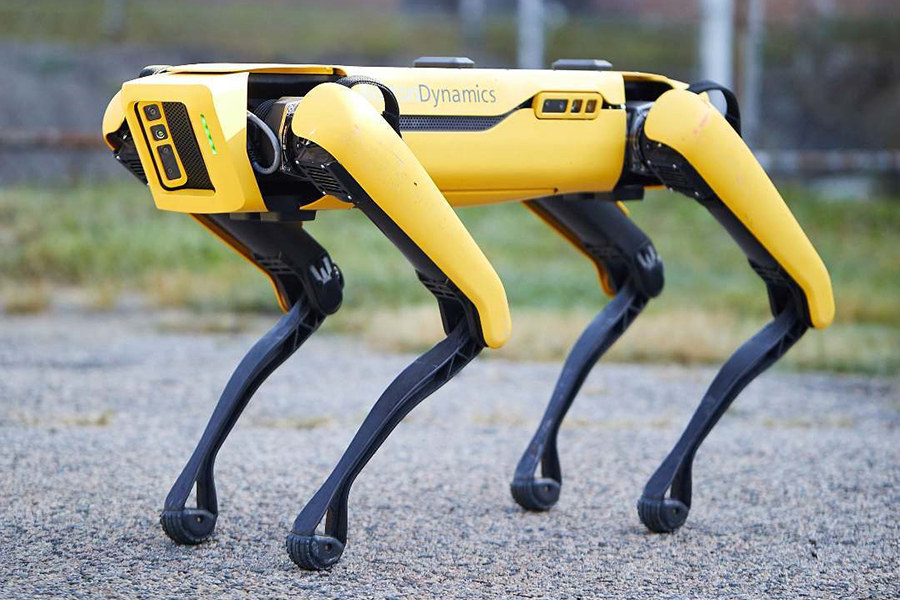
\includegraphics[height=1.33in]{images/spot.jpg}
    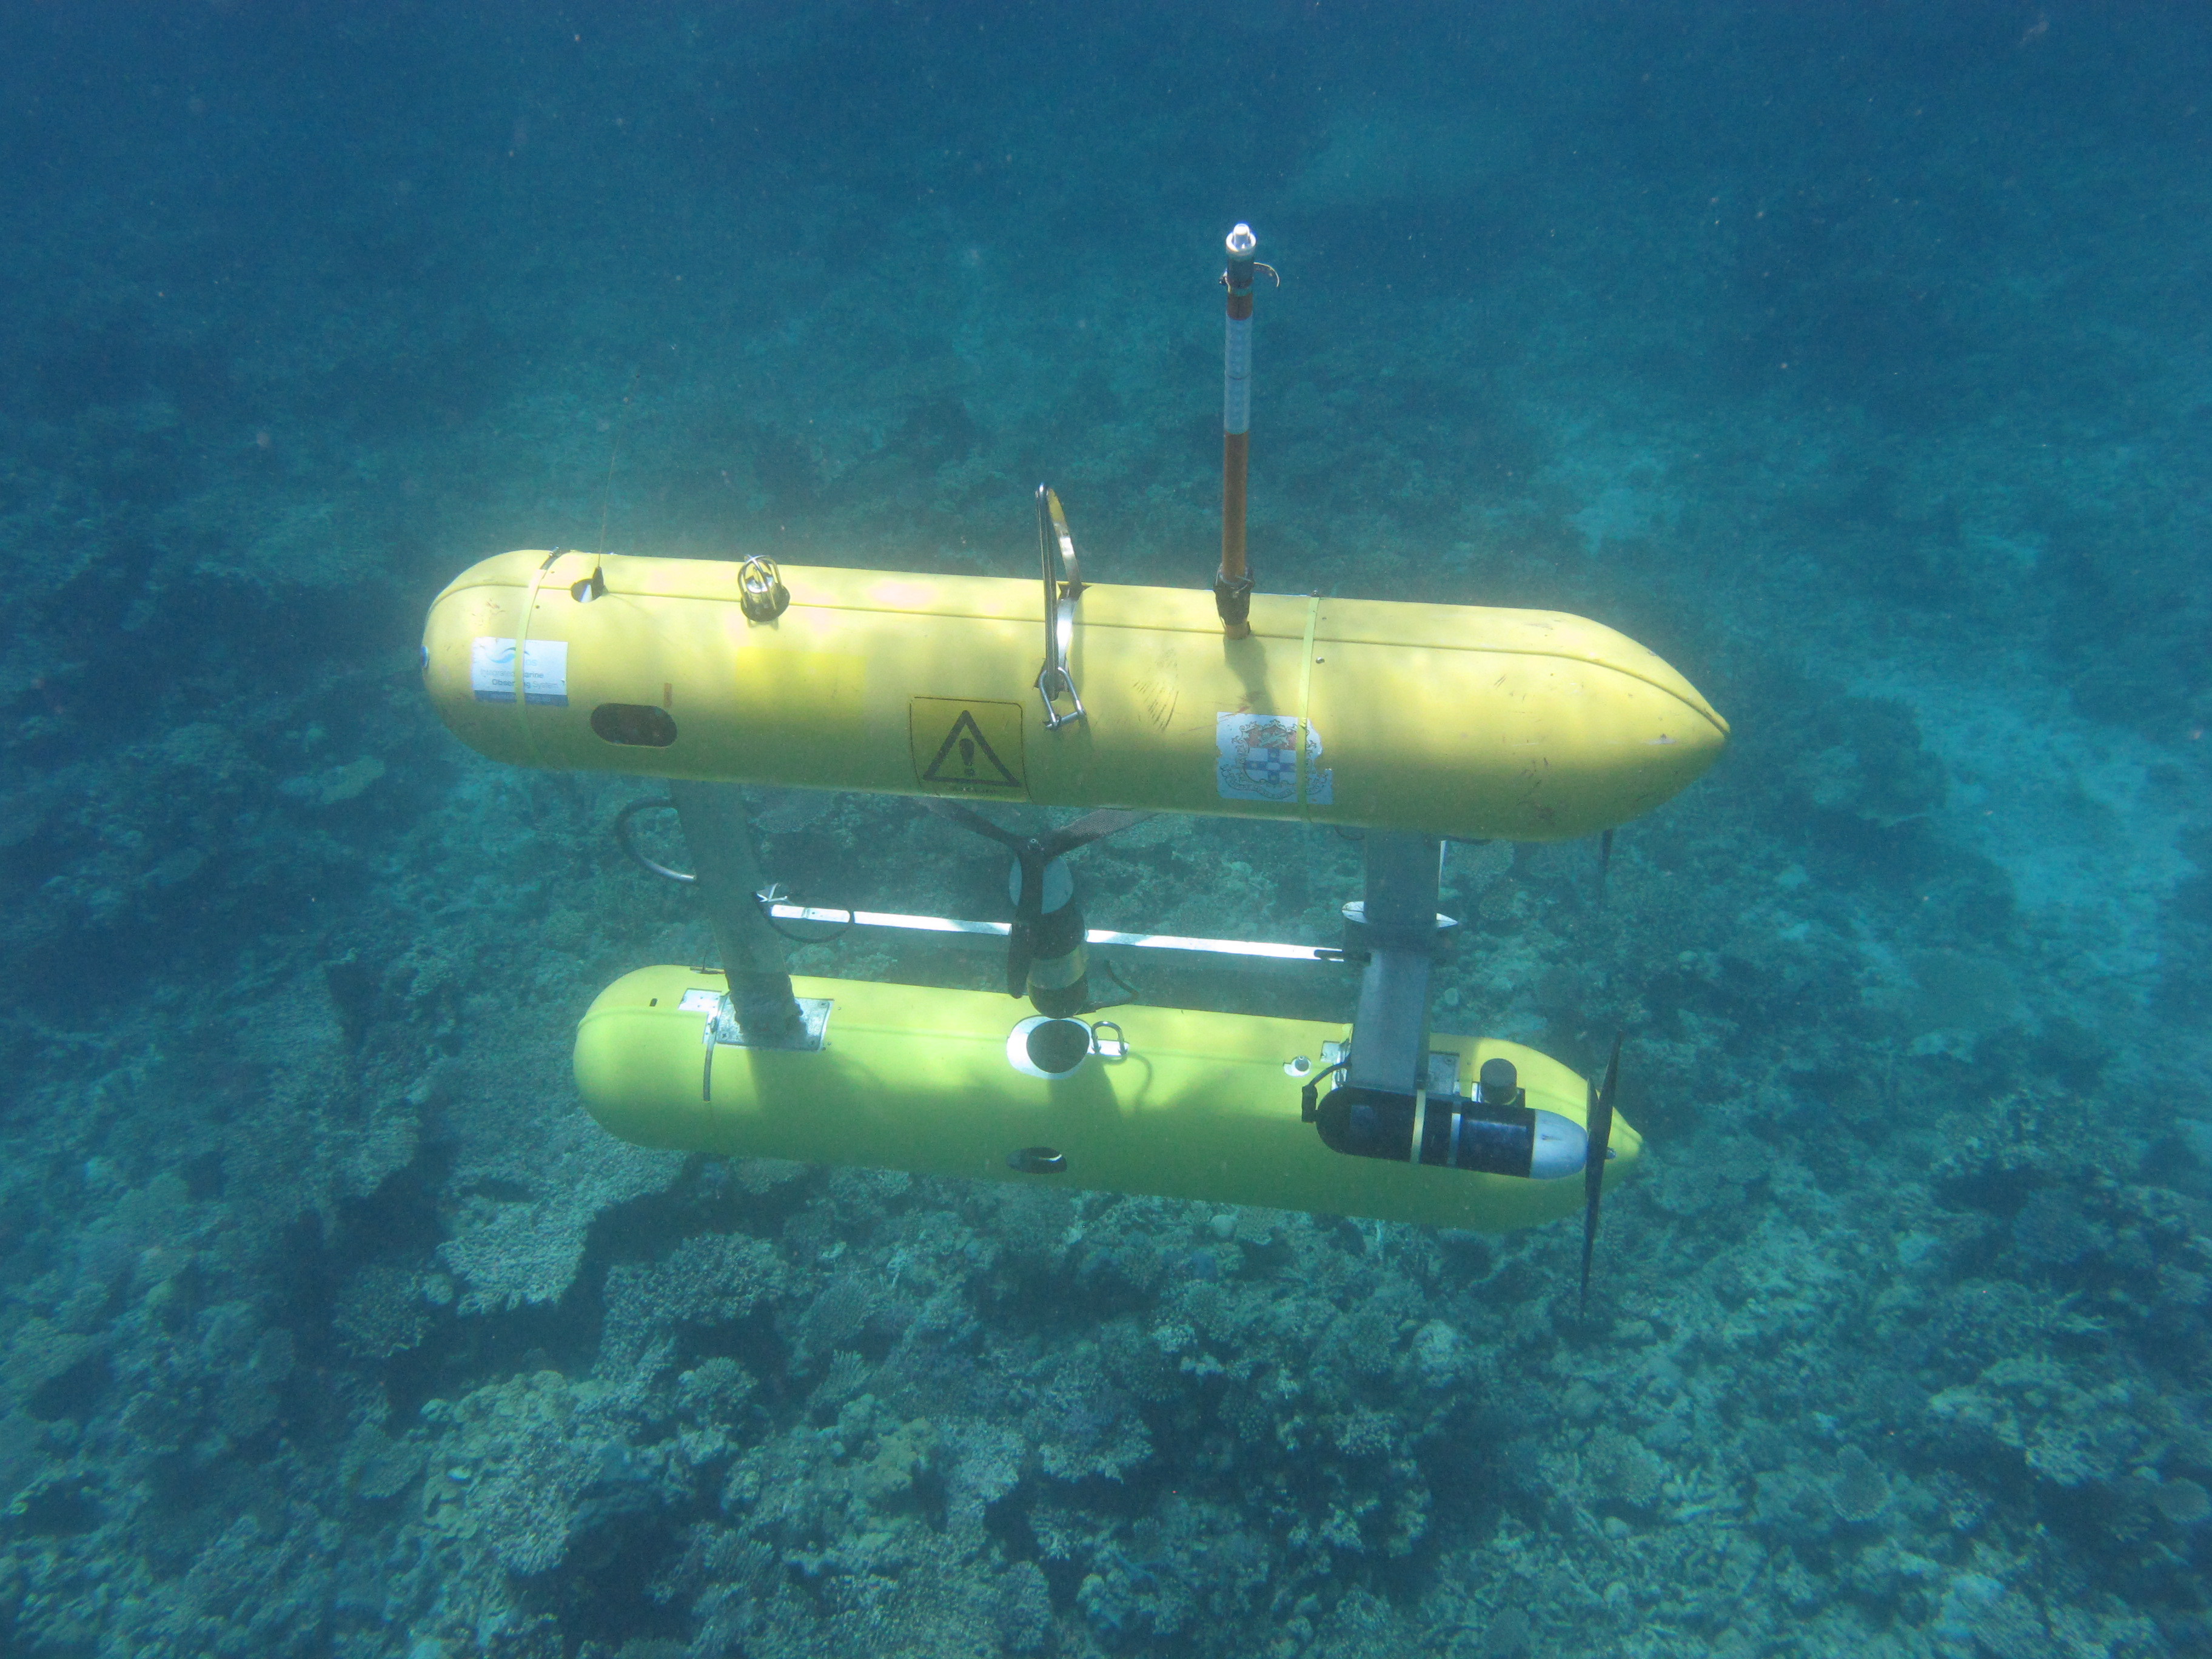
\includegraphics[height=1.33in]{images/rov_sirius.jpg}
    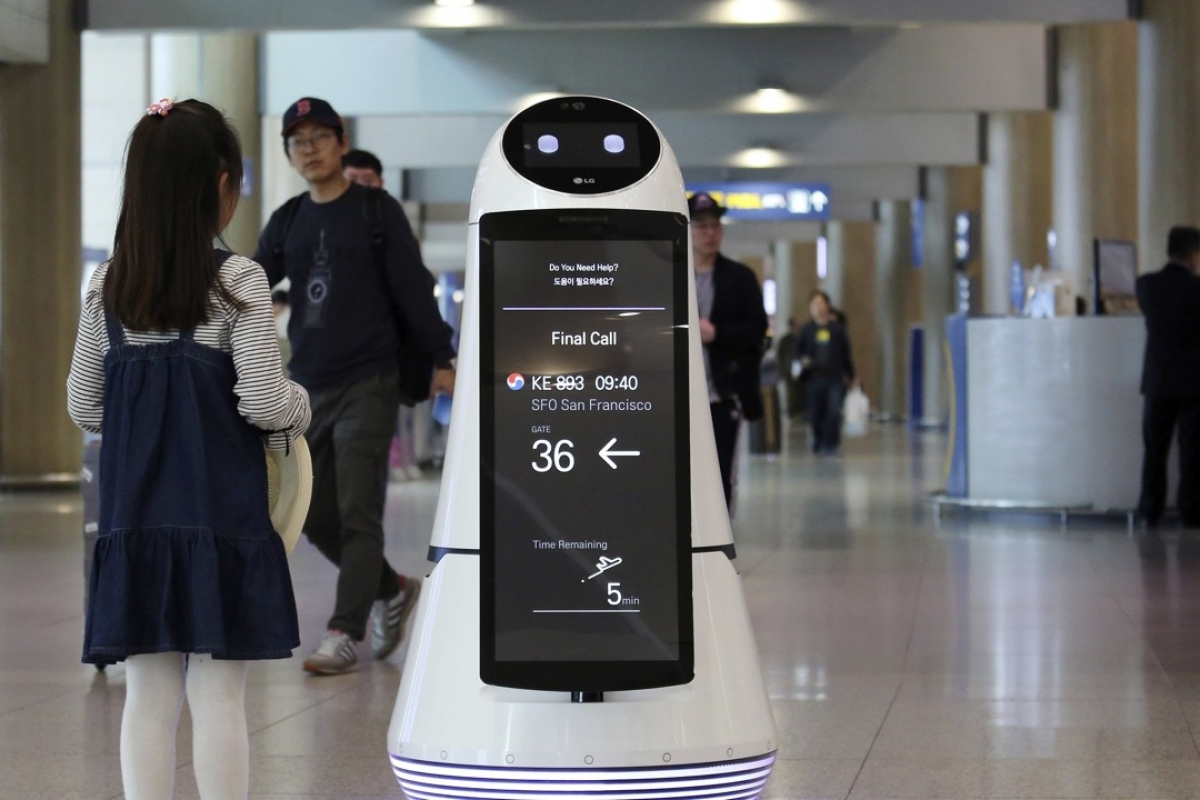
\includegraphics[height=1.33in]{images/troika.jpg}
    \caption[Examples of robots that operate in unconstrained spaces.]{Autonomous mobile robots are increasingly operating in unconstrained environments, which can be characterised by uneven terrain, weak GPS signal, or crowds of people. An important challenge for the broader adoption of these types of mobile robots is navigational capabilities, which relies fundamentally on mapping and localisation. \textit{Left}: Spot by Boston Dynamics. \textit{Center}: AUV Sirius by the Australian Center for Field Robotics. \textit{Right}: Troika by LG, currently deployed at Incheon International Airport in Seoul.}
\end{figure}


One might question the practicality of using image data for these tasks when great success has been found with more specialised sensing modalities; motion estimation for example is typically addressed with inertial sensor measurements or Global Positioning System (GPS) receivers. Other robotic systems employ lidar, acoustic range-finding, time-of-flight cameras or structured-light cameras to gain access to 3D models of the environment. Cameras however, can often offer superior qualities in size, weight, cost, power consumption, and they deliver a rich, highly detailed representation of the world. Furthermore, unlike \textit{active} sensor technologies which sense the world by `illuminating' it, cameras are \textit{passive} sensors, meaning they do not interfere with one another and can be employed in a more diverse range of environments. Thanks to their ability to adjust their exposure period, aperture size and sensor gain, cameras are also highly capable in a variety of lighting conditions and environments. 

Furthermore, the applications of visual odometry extend beyond the context of SLAM algorithms. For example, a multi-rotor Unmanned Aerial Vehicle (UAV) can fuse measurements from inertial and visual measurements to hover in place in GPS denied environments. Outside of the field of robotics, Augmented Reality (AR) applications are employing visual odometry and SLAM to render virtual 3D models in real time on top of camera feeds. Proença \cite{proenca2018rgbd} envisages an AR application that employs visual odometry to guide an operator through a contaminated nuclear facility, whilst rectifying existing 3D models of the facility. The adversities of installing guidance and navigation infrastructure in such facilities can be extrapolated to cases such as planetary rovers and Remotely Operated Underwater Vehicles (ROVs).


\subsection{Computational Imaging}

Despite the many advantages of visual perception in robotics, we should not discount the inherent trade off bound to cameras by the laws of optics. Each pixel in a modern digital camera sensor integrates the number of arriving photons in order to form an image. A lens can help concentrate rays from a larger area through the cameras aperture; the larger the aperture, the more light is received at the sensor, allowing fine control over the exposure. A larger aperture diameter however also gives rise to a shallower depth of field, which can be used to produce aesthetically pleasing images in photography, but limits the regions of the image where computer algorithms perform well. Similarly, more light can be collected by integrating photons over a longer period of time, but in robotics where the camera tends to be moving, this leads to motion blur and reduced image clarity.

In response to these limitations, \textit{computational photography} has catapulted modern imaging into an age where optics, algorithms, sensors and illumination are designed in coordination with one another. Take modern smart-phones as an example, with their relatively slow lenses, small sensors, and cheap optics. In comparison to the enormous lenses and excellent sensors of their DSLR cousins, smart-phones should by all rights produce lower quality images. Modern smart-phones however benefit from powerful CPUs, hardware-accelerated graphics, and an entire community of software engineers working on image processing algorithms. Many of the effects that were once unique to expensive imaging devices are now being replicated on smartphones. Low light imaging is enhanced using algorithms such as Google's `Night Sight', and more recently machine learning been used to improve clarity, colour accuracy and signal-to-noise ratios. Bokeh, an effect that is typically difficult to achieve on a wide lens is now replicated with `Portrait Mode', another smartphone feature employing a range of computational imaging techniques.

This work similarly adopts computational imaging as an approach to visual odometry. Humans are exceptionally well adapted to tasks involving visual motion and depth perception - our two eyes allow us to process the 3D geometry of the scene, while our learned experiences are often able to fill in the gaps where geometric information is insufficient or unavailable. Image processing algorithms are not equipped with this same kind of human intuition, and so the deceptively complex task of estimating the 3D structure of a scene from a sequence of images continues to attract attention from the computer vision community \cite{dansereau2011plenopticflow,nister2004vo,gakne2018scale,zhou2019scale}. 

The price of camera components is decreasing while image quality continues to improve, not only making cameras an attractive perception module for autonomous robotics, but also spurring the popularity of multiple-view imaging. Embracing this idea, this work develops an algorithm that performs visual odometry by taking advantage of the rich geometric information exposed when using multiple views. Thus, the vocabulary and concepts from the literature on light field imaging are adopted broadly throughout this work. More broadly however, the principle underpinning much of this thesis is that novel imaging devices that break away from the traditional pinhole model of the camera have vast implications in the field of machine vision. We need not look any further than the animal kingdom to see why this is true - the biological eye is estimated to have evolved independently no fewer than 50 times, each variant acutely adapted to the particular set of challenges in their environment. The diversity and evolutionary ingenuity in biological visual perception systems prompts an important question in robotics and computer vision - how best should we equip robots to see the world given a particular set of challenges and environments? In this thesis, a camera array which is a simple yet versatile extension of the stereo camera is used to develop the algorithms that address the visual odometry and depth reconstruction problems. 



\section{Problem Statement}

There is a well established library of solutions addressing the visual odometry and depth reconstruction problems. Some use closed form solutions that directly solve for geometry and ego-motion, while others, like this work utilise a data-driven approach to indirectly model visual odometry. These two families of algorithms, which will be referred to as the \textit{geometric} and \textit{data-driven} approaches respectively throughout this work, form two crucial touchstones from which our pipeline will be evaluated. 

An important challenge addressed in this work that is absent in the present literature of either family, is the ability to perform visual odometry using an \textit{uncalibrated} camera array. Robots operating in challenging environments are frequently subjected to destabilising effects such as thermal expansion, vibration and shock, frequently rendering calibrations invalid. Multiple-view geometry, which is harnessed by the \textit{geometric} family of algorithms, is materially dependent on knowing the orientation and position of the cameras; rotating a camera even a few arc-seconds from its calibrated position results in a disproportionally magnified error in the image being formed, especially in large, open spaces where field robotics tend to operate. 

Existing \textit{data-driven} approaches on the other hand, have typically used monocular or stereo imagery, overlooking the richness of light field imagery as a possibility for improving robustness and accuracy. Within the data-driven family of algorithms, a relatively new \textit{unsupervised} approach has emerged, cleverly piecing together the available information to learn visual odometry from raw footage alone. The unsupervised nature of this approach means that the model calibrates itself in a fashion, learning from raw data to produce ego-motion predictions. Unsupervised machine learning makes `online-learning' possible, in which models take advantage of new data becoming available in-situ, improving performance and building robustness to different environments. Most importantly however, unsupervised models are able to adapt to errors in the calibration of the equipment without requiring hand-labelled data to supervise the learning process. A self-calibrating and adaptive perception module which is robust to adverse effects is an attractive capability in robotics. Once again however, existing unsupervised algorithms have not been applied to light field data, prompting a natural, yet important next step which is the subject of this work: combining the richness of light field data with the self-calibrating capabilities of unsupervised learning algorithms to perform visual odometry.



\section{Contributions}
This work builds on existing data-driven approaches, suggesting an adaptation of conventional 2D machine learning algorithms to enable unsupervised learning on light field data. Specifically, we suggest two novel variants of an existing algorithm that enables the ingestion of 4D imagery. Furthermore, we describe three encodings of the light field that presents 4D data as 2D slices, from which convolutional networks are able to learn the tasks of depth- and pose-estimation. The three light field encodings are compatible with both variants of the proposed algorithm, allowing for a direct comparison between input methods. We demonstrate that our algorithm out-performs existing monocular approaches for depth and visual odometry, reinforcing the benefits of light field technology in robotic imaging.

\textbf{TODO: Bullet list of contributions}

\section{Outline}
Concepts from computer vision, machine learning and light field imaging are used heavily throughout this thesis, and \textbf{Chapter 2} begins by providing an overview of the relevant background information. On the subject of computer vision, it describes the pinhole model of the camera, the fundamentals of multiple view geometry, and develops intuition relevant to light field imaging. Machine learning is presented as an approach to solving computer vision problems, with emphasis directed towards convolutional neural networks, as an algorithm that continues to gain popularity in image based problems.

The existing approaches for performing visual odometry and depth estimation are reviewed in \textbf{Chapter 3}, presented in two categories: geometric approaches which rely on directly modeling movement through 3D space, and machine learning approaches which take advantage of massive datasets to build resilient, data-driven solutions.

\textbf{Chapter 4} introduces a novel light-field based algorithm for simultaneously learning depth and pose. Though algorithms have been proposed in previous work that perform the two tasks either monocularly or with stereo camera pairs, this thesis differs in the use of light-field imagery to gain improved access to geometric information in the scene. While previous work has benefitted from large scale open source datasets, similar pose-stamped footage does not exist publicly for camera arrays. The acquisition of such a dataset thus forms one of the objectives of this thesis, the methodology for which is discussed in the chapter.

\textbf{Chapter 5}, presents the results from initial experiments using the pipeline described in Chapter 4, performed on both the early dataset and the open source KITTI dataset \cite{dataset-kitti}. The early challenges and milestones are discussed, and a qualitative discussion on the successes, failure modes, and future directions is presented. 

% An updated research proposal is provided in \textbf{Chapter 6} with emphasis placed on the expected milestones in the remainder of the project. 